\documentclass[unicode,10pt]{beamer}
\usetheme{ttiposter}

\usepackage{luatexja}
\usepackage{luatexja-fontspec}
\usepackage{geometry}
\usepackage{graphicx}
\usepackage{multicol}
\usepackage{subcaption}
\captionsetup{compatibility=false}

\setmainjfont{ipagp.otf}
\beamertemplatenavigationsymbolsempty

\geometry{a4paper,portrait,left=2truemm,width=206truemm,right=2truemm}
\newlength{\mycolumnwidth}
\setlength{\mycolumnwidth}{0.495\textwidth}
\newlength{\mytitlefigureheight}
\setlength{\mytitlefigureheight}{1.5em}

\newcommand{\arrow}{\textcolor{ttiblue}{\textbf{→}}\hspace{1ex}}
\newcommand{\itemtitle}[1]{#1\\}
\newcommand{\fire}[1]{\textcolor{red}{\textbf{#1}}}
\newcommand{\doublecolumns}[4]{
    \begin{minipage}[t]{#1}
      #2
    \end{minipage}
    \begin{minipage}[t]{#3}
      #4
    \end{minipage}}

\title{レーティング予測によるフォントを基盤としたレビュー解析}
\institute{豊田工業大学 知能数理研究室}
\author{外山 洋太, 三輪 誠, 佐々木 裕}
\date{\today}



\begin{document}
\begin{frame}[t]
\vspace{-1em} % HACK

\begin{columns}[onlytextwidth,t]
  \begin{column}{1.1\mycolumnwidth}
    \begin{block}{背景と目的}
      \begin{itemize}
        \item 対象タスク:表意・表語文字を含む言語におけるレーティング予測
        \item 応用例:企業における文書からの商品の評判分析
        \item 目的:文字の表層情報を利用したレーティング予測の実現
      \end{itemize}
    \end{block}
    \begin{figure}
      \begin{subfigure}{0.5\linewidth}
        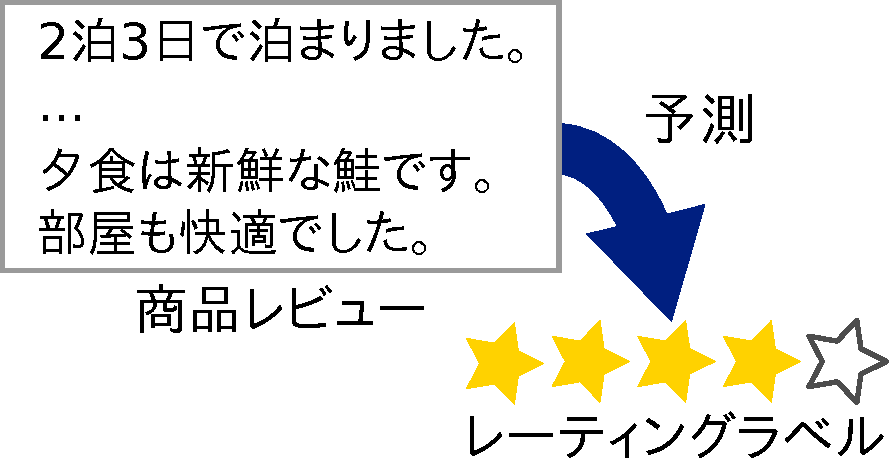
\includegraphics[width=\linewidth]{fig/review.pdf}
      \end{subfigure}%
      ~
      \begin{subfigure}{0.45\linewidth}
        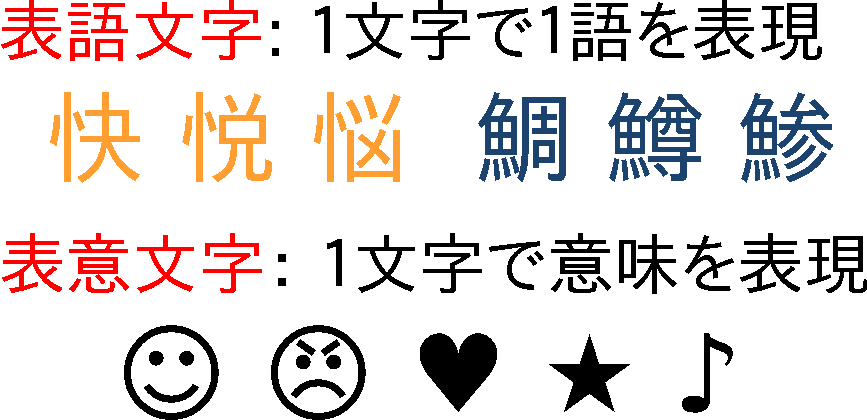
\includegraphics[width=\linewidth]{fig/logogram_and_ideogram.pdf}
      \end{subfigure}
    \end{figure}
  \end{column}
  \begin{column}{0.9\mycolumnwidth}
    \begin{block}{関連研究}
      \begin{itemize}
        \item \itemtitle{Hierarchical Attention Network (HAN) \cite{yang16}}
          \begin{itemize}
            \item Attention構造付きのRecurrent Neural Network (RNN)を用いた
                  文書分類モデル
            \item 文字または単語から文、文書までの階層構造を利用
          \end{itemize}
          \arrow \fire{文字の表層情報の利用ができていない}
        \item \itemtitle{Radical-Enhanced Chinese Character Embedding
                         \cite{sun14}}
          \begin{itemize}
            \item 漢字-部首辞書を利用した漢字埋め込みの生成手法
            \item 対象タスクと漢字の部首当てについて同時に学習
          \end{itemize}
          \arrow \fire{漢字-部首辞書が余分に必要}
      \end{itemize}
    \end{block}
  \end{column}
\end{columns}


\begin{columns}[onlytextwidth,t]
  \begin{column}{1.1\mycolumnwidth}
    \begin{block}{提案手法}
      \begin{itemize}
        \item 入力:フォント画像で表現されたレビュー
        \item 出力:予測したレーティングラベル
        \item 特徴
          \begin{itemize}
            \item \fire{フォント画像}から文字の意味情報を抽出
            \item HAN\cite{yang16}の手法を基に文字からの\fire{文書の階層構造}を利用
          \end{itemize}
        \item 予測過程
          \begin{enumerate}
            \item 畳み込みNN (LeNet)によりフォント画像を文字埋め込みを生成
            \item 文字から単語、単語から文、文から文書へ階層的に
                  Gated Recurrent Unit (GRU)によるRNNを用いて埋め込みを生成
            \item 文書埋め込みからラベルを予測
          \end{enumerate}
      \end{itemize}
      \begin{figure}
        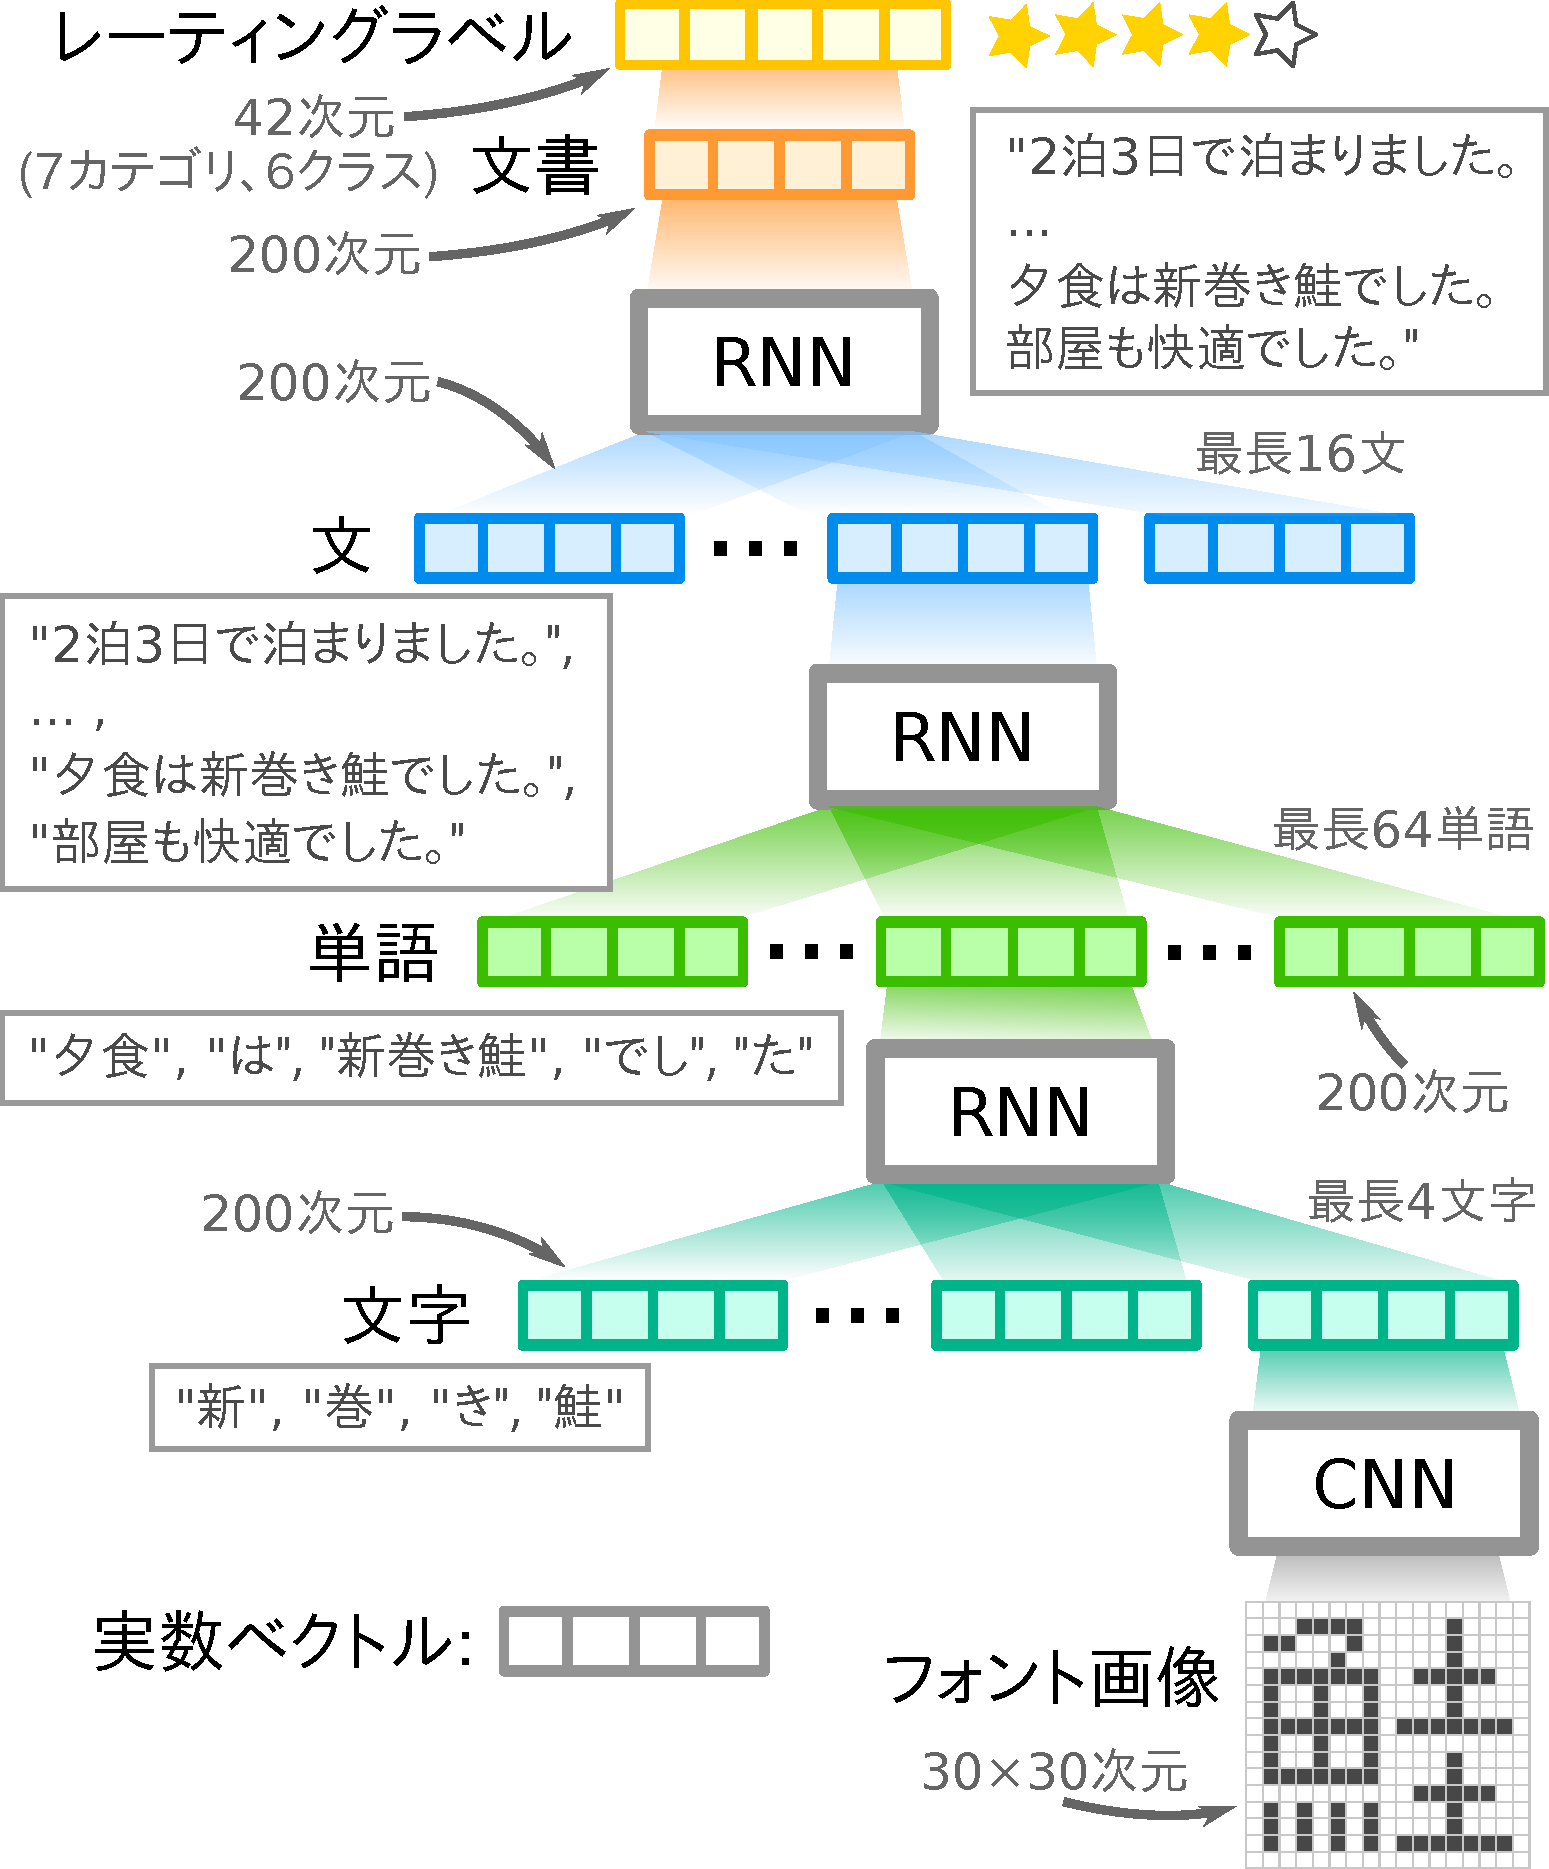
\includegraphics[width=0.85\linewidth]{fig/fcwsd.pdf}
      \end{figure}
      \vspace{-1ex} % HACK
      \begin{itemize}
        \item アテンション構造 \cite{yang16}
          \hspace{-8em} % HACK
          \begin{minipage}[t]{0.4\linewidth}
            \begin{gather*}
              u_i = \tanh (W h_{i} + b) \\
              \alpha_i = \frac{\exp (u^T_i u_{context})}
                              {\sum_i \exp (u^T_i u_{context})} \\
              \hat{h} = \sum_i \alpha_i h_i
            \end{gather*}
          \end{minipage}
          \begin{minipage}[t]{0.1\linewidth}
            \begin{gather*}
              \begin{cases}
                u_{context} : \text{文脈ベクトル} \\
                \alpha_i : \text{アテンション} \\
                h_i : \text{下の階層の埋め込み} \\
                \hat{h} : \text{上の階層の埋め込み} \\
                W, b : \text{線形層のパラメータ}
              \end{cases}
            \end{gather*}
          \end{minipage}
      \end{itemize}
    \end{block}
  \end{column}

  \begin{column}{0.9\mycolumnwidth}
    \begin{block}{実験}
      \begin{itemize}
        \item \itemtitle{実験設定}
          \begin{itemize}
            \item 7カテゴリにおける0〜5点のレーティング予測
            \item データセット:楽天トラベルのレビュー310,000件 \\
                  (訓練データ: 300,000件、テストデータ: 10,000件)
          \end{itemize}
      \end{itemize}

      \begin{minipage}[t]{0.55\linewidth}
        \begin{itemize}
          \item \itemtitle{結果}
            \begin{itemize}
              \item 従来手法(パラグラフベクトルを応用した手法)より高い正答率
            \end{itemize}
        \end{itemize}
      \end{minipage}%
      \begin{minipage}[t]{0.4\linewidth}
        \begin{table}
          \centering
          \begin{tabular}{l | r}
            手法 & 正答率 \\
            \hline
            従来手法\cite{me16} & 0.503        \\
            提案手法            & \fire{0.524} \\
          \end{tabular}
        \end{table}
      \end{minipage}

      \begin{itemize}
        \item 高いアテンションが付く表現
          \begin{itemize}
            \item 「食」、「部屋」、「風呂」等の\fire{カテゴリ}を表すもの
            \item 「広」、「満」、「良」、「悪」等の\fire{評価}を表すもの
            \item 「は」、「が」、「も」等の助詞
          \end{itemize}
      \end{itemize}

      \begin{figure}
        \centering
        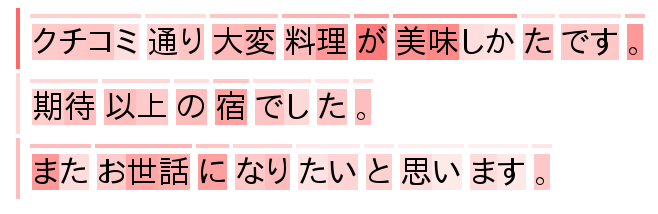
\includegraphics[width=0.9\linewidth]{fig/review_1.png}
        \caption*{レビューのアテンション例 (1)}
      \end{figure}

      \begin{figure}
        \centering
        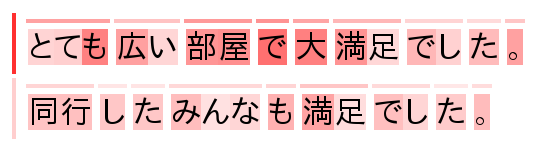
\includegraphics[width=0.8\linewidth]{fig/review_2.png}
        \caption*{レビューのアテンション例 (2)}
      \end{figure}
    \end{block}

    \begin{block}{まとめ}
      \begin{itemize}
        \item フォント画像を用いたレーティング予測及びレビュー解析の手法を提案
        \item 提案手法による従来手法\cite{yang16}より高い正答率
        \item アテンションの可視化によるレビューの解析
        \item \itemtitle{今後の予定}
          \begin{itemize}
            \item フォント画像に対するアテンションの可視化の実装
          \end{itemize}
      \end{itemize}
    \end{block}

    \vspace{2ex} % HACK
    参考文献
    \bibliographystyle{jplain}
    \begin{thebibliography}{9}
      \bibitem{yang16}
        Zichao Yang et al.,
        Hierarchical Attention Networks for Document Classification.
        NAACL 2016, 2016.
      \bibitem{sun14}
        Yaming Sun et al.,
        Radical-Enhanced Chinese Character Embedding.
        ICONIP 2014, 2014.
      \bibitem{me16}
        外山洋太ら,
        文書・文間及びカテゴリ間の関係を考慮したレーティング予測.
        豊田工業大学 学士論文.
    \end{thebibliography}
  \end{column}
\end{columns}

\end{frame}
\end{document}
